% ch_lp_types.tex  —  Chapter: Linear programming: formulation and application to ship configuration design
% Content only — compiled via main.tex
% Figures in fig/, code in code/
\chapter{Linear programming: formulation and application to ship configuration design}
\label{ch:lp-intro}

In the previous chapter, ship size and speed were treated as continuous
production factors, and the optimal combination followed from setting a
derivative to zero. Most design decisions are not that unconstrained: a
designer choosing how much cargo to load, how many cabins of each type to
build, or how to lay out equipment on a deck is working against explicit
limits on weight, area, length, or capacity. \emph{Linear programming} (LP)
is the natural first tool for this class of problem: it handles many
decision variables and many constraints simultaneously, as long as the
objective and the constraints are linear in the decision variables.

This chapter introduces the structure of a linear program, develops a
disciplined approach to formulating design problems mathematically, and
applies both to a recurring class of ship design problem: allocating a
scarce resource (deck area, side length, tank volume) across a set of
competing uses. The cabin arrangement problem, used throughout, is a small
but genuine instance of what is generally called a \emph{general
arrangement} or \emph{configuration} problem.

\section{The structure of a linear program}

\subsection{Decision variables, objective function, and constraints}

A linear program has three ingredients: a set of \emph{decision variables}
$x_1, x_2, \ldots, x_n$ representing quantities the designer controls; a
linear \emph{objective function} to be maximized or minimized; and a set of
linear \emph{constraints} that the variables must satisfy. In maximization
form,
\begin{align}
  \max \quad & Z = c_1 x_1 + c_2 x_2 + \cdots + c_n x_n \label{eq:lp-obj}\\
  \text{s.t.} \quad & a_{11}x_1 + a_{12}x_2 + \cdots + a_{1n}x_n \leq b_1 \notag\\
  & \qquad\qquad \vdots \notag\\
  & a_{m1}x_1 + a_{m2}x_2 + \cdots + a_{mn}x_n \leq b_m \notag\\
  & x_1, x_2, \ldots, x_n \geq 0. \notag
\end{align}
The coefficients $c_j$ translate a unit of variable $j$ into objective
value; the coefficients $a_{ij}$ translate a unit of variable $j$ into
consumption of resource $i$; and $b_i$ is the amount of resource $i$
available. The non-negativity constraints are not optional bookkeeping —
they reflect that most design quantities (tonnes of cargo, number of
cabins, square metres of deck) cannot be negative.

\subsection{Standard form}
\label{sec:standard-form}

It is convenient to fix a reference form for the model above: a
maximization objective, all functional constraints written as
$\leq$, and non-negative right-hand sides $b_i$. This is the \emph{standard
form} of an LP. A minimization problem, a $\geq$ constraint, or an equality
constraint can always be rewritten into this form (multiply through by
$-1$, or split an equality into two inequalities), so standard form loses
no generality; it is simply a common reference point that makes it
possible to talk about "the" constraint matrix $A$, objective vector $c$,
and right-hand side vector $b$ without restating conventions every time.

\subsection{The defining assumptions}
\label{sec:lp-assumptions}

Linearity is a strong assumption, and it is worth being explicit about
what it requires, because the cases where this assumptions fail will motivate most of the methods covered later in the course.

\begin{description}
  \item[Proportionality.] The contribution of variable $x_j$ to the
  objective and to each constraint is directly proportional to $x_j$ — no
  economies of scale, no fixed costs, no threshold effects. When this
  fails (as it typically does for the diminishing returns of speed and size on the annual transport capacity, or propulsion power as a function of
  speed, Chapter~\ref{ch:lp-intro}\nobreak\ notwithstanding), the model
  becomes non-linear.
  \item[Additivity.] The total effect of several variables is the sum of
  their individual effects — no interaction terms. This is what allows
  the objective and constraints to be written as simple sums.
  \item[Divisibility.] Decision variables may take any non-negative real
  value, including fractions. A solution of $x_1 = 149.7$ cabins is
  mathematically fine even though it is not physically buildable. When
  variables must be integer (a number of cabins, a yes/no equipment
  choice), the problem becomes an integer or mixed-integer program.
  \item[Certainty.] All coefficients $c_j$, $a_{ij}$, and $b_i$ are known
  with certainty. When freight rates, fuel prices, or demand are
  uncertain, the deterministic LP is at best a first approximation, and
  the methods introduced later under decisions under uncertainty become
  relevant.
\end{description}

Divisibility deserves a preliminary remark, because the cabin problem
worked later in this chapter happens to have an integer optimal solution
even though it is formulated as a continuous LP. That is a coincidence of
the particular numbers involved, not a general property of LP relaxations
of integer problems, and it should not be relied upon in general.

However, if you do get an integer solution to a problem without the integer constraints (the so-called \textit{relaxed problem}, this solution is also valid for the integer-constrained problem. This reflects a general principle that we do not improve our solution by adding constraints.

\section{A first worked example: cargo mix on a supply vessel}
\label{sec:cargo-mix}

\subsection{Problem description and data}

Consider a vessel loading two cargo types, cement and brine, for a single
voyage (so this is evidently a very simplified problem). Each tonne of cargo earns a different freight rate, occupies adifferent stowage volume (including any tank or hold overhead), and the vessel is subject to a deadweight limit, a hold volume limit, and a contractual minimum quantity of cement. The decision is how many tonnes of each cargo type to load.

\begin{center}
\begin{tabular}{@{}llll@{}}
\toprule
Quantity & Symbol & Value & Unit \\
\midrule
Weight of cement loaded & $x_1$ & decision variable & t \\
Weight of brine loaded & $x_2$ & decision variable & t \\
Freight rate, cement & $c_1$ & 2 & kEUR/t \\
Freight rate, brine & $c_2$ & 3 & kEUR/t \\
Max.\ cargo deadweight & $b_1$ & 2500 & t \\
Specific volume, cement & $a_{21}$ & 1.5 & m$^3$/t \\
Specific volume, brine & $a_{22}$ & 3 & m$^3$/t \\
Max.\ available hold volume & $b_2$ & 4500 & m$^3$ \\
Min.\ required cement & $b_3$ & 500 & t \\
\bottomrule
\end{tabular}
\end{center}

\subsection{Formulation}

\begin{align}
  \max \quad & Z = 2x_1 + 3x_2 \label{eq:cargomix}\\
  \text{s.t.} \quad & x_1 + x_2 \leq 2500 \quad \text{(deadweight)} \notag\\
  & 1.5x_1 + 3x_2 \leq 4500 \quad \text{(volume)} \notag\\
  & x_1 \geq 500 \quad \text{(minimum cement)} \notag\\
  & x_1, x_2 \geq 0. \notag
\end{align}

\subsection{Graphical solution}

With two variables, the feasible region and the optimum can be found
graphically. Each constraint defines a half-plane; their intersection is
the feasible region, a polygon with four corners: $(500,0)$, $(2500,0)$,
$(2000,500)$, and $(500,1250)$. Because the objective function is linear,
its maximum over a polygon is always attained at a corner (this is the
geometric fact the Simplex method exploits algebraically, in
Section~\ref{sec:bridging}). Evaluating $Z = 2x_1+3x_2$ at each corner:

\begin{center}
\begin{tabular}{@{}lccc@{}}
\toprule
Corner & $x_1$ & $x_2$ & $Z$ \\
\midrule
A & 500 & 0 & 1000 \\
B & 2500 & 0 & 5000 \\
C & 2000 & 500 & \textbf{5500} \\
D & 500 & 1250 & 4750 \\
\bottomrule
\end{tabular}
\end{center}

\noindent The optimum is at corner C, where the deadweight and volume
constraints are both binding: $x_1^\ast = 2000$~t of cement, $x_2^\ast =
500$~t of brine, $Z^\ast = 5500$~kEUR. Note that the minimum-cement
constraint $x_1 \geq 500$ is \emph{not} binding at the optimum — the
optimal cement load is already four times the contractual minimum. We will return to the importance of identifying \textit{binding} constraints ion the post-solution analysis.

\begin{center}
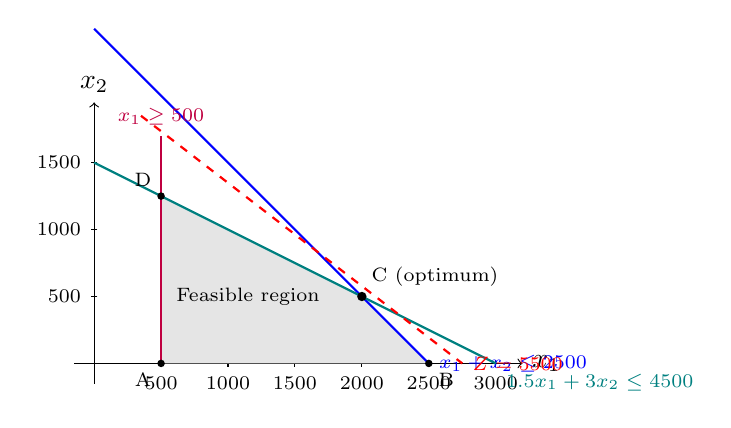
\begin{tikzpicture}[scale=0.85]
  % axes
  \draw[->] (-0.3,0) -- (6.4,0) node[right] {$x_1$};
  \draw[->] (0,-0.3) -- (0,3.9) node[above] {$x_2$};
  \foreach \x/\lbl in {1/500,2/1000,3/1500,4/2000,5/2500,6/3000}
    \draw (\x,0.05) -- (\x,-0.05) node[below,font=\scriptsize] {\lbl};
  \foreach \y/\lbl in {1/500,2/1000,3/1500}
    \draw (0.05,\y) -- (-0.05,\y) node[left,font=\scriptsize] {\lbl};

  % feasible region (scale: 1 unit = 500 t)
  \fill[gray!20] (1,0) -- (5,0) -- (4,1) -- (1,2.5) -- cycle;

  % constraint lines
  \draw[thick,blue] (0,5) -- (5,0) node[right,font=\scriptsize,blue] {$x_1+x_2\leq 2500$};
  \draw[thick,teal] (0,3) -- (6,0) node[below right,font=\scriptsize,teal] {$1.5x_1+3x_2\leq 4500$};
  \draw[thick,purple] (1,0) -- (1,3.4) node[above,font=\scriptsize,purple] {$x_1\geq 500$};

  % iso-profit line through the optimum: 2x1+3x2 = 5500
  \draw[dashed,red,thick] (0.7,3.7) -- (5.5,0) node[right,font=\scriptsize,red] {$Z=5500$};

  % vertices
  \fill (1,0) circle (1.6pt) node[below left,font=\scriptsize] {A};
  \fill (5,0) circle (1.6pt) node[below right,font=\scriptsize] {B};
  \fill (4,1) circle (2pt) node[above right,font=\scriptsize] {C (optimum)};
  \fill (1,2.5) circle (1.6pt) node[above left,font=\scriptsize] {D};

  \node at (2.3,1.0) [font=\scriptsize] {Feasible region};
\end{tikzpicture}
\end{center}

\section{A structured approach to formulating design problems}
\label{sec:structured-formulation}

\subsection{Why structure matters}

The cargo-mix example was formulated directly, with named variables
$x_1$, $x_2$. This works for two variables but breaks down as soon as a
problem involves a set of cargo types, cabin types, or equipment items
whose size is not fixed in advance. A structured formulation — organized
into \emph{sets}, \emph{parameters}, \emph{variables}, and \emph{model} —
scales to any number of items, communicates the model unambiguously to a
reader who was not in the room when it was built, and can be checked for
correctness before a single line of code is written. It also, done well,
gives a near one-to-one correspondence between the mathematical statement
and its implementation, which is the single largest time-saver when
debugging a model that does not solve as expected.

Further, keeping a strict division between the generic model and the data set(s) corresponding to the parameters of the model enables the easy reuse of the same model across many cases and datasets. This is also helpful in model development. You can start with a very simple model just for testing purposes, and then exand this to real cases without touching the model itself.

\subsection{Sets, parameters, variables, and model}

Recast in this structure, the cargo-mix problem reads:

\medskip
\noindent\textbf{Sets}
\begin{align*}
  K  && \text{set of cargo types (cement, brine), indexed by } k
\end{align*}

\noindent\textbf{Parameters}
\begin{align*}
  R_k & && \text{freight rate for cargo type } k \text{ (kEUR/t)} \\
  V_k & && \text{stowage volume per tonne of cargo type } k \text{ (m}^3\text{/t)} \\
  W^{\text{MAX}} & && \text{maximum deadweight (t)} \\
  U^{\text{MAX}} & && \text{maximum hold/tank volume (m}^3\text{)} \\
  Q_k^{\text{MIN}} & && \text{minimum quantity of cargo type } k \text{ (t)}
\end{align*}

\noindent\textbf{Variables}
\begin{align*}
  x_k & && \text{tonnes of cargo type } k \text{ loaded}
\end{align*}

\noindent\textbf{Model}
\begin{align}
  \max \quad & \sum_{k \in K} R_k x_k \notag\\
  \text{s.t.} \quad & \sum_{k \in K} x_k \leq W^{\text{MAX}} \notag\\
  & \sum_{k \in K} V_k x_k \leq U^{\text{MAX}} \notag\\
  & x_C \geq Q_C^{\text{MIN}} \notag\\
  & x_k \geq 0, \quad k \in K \notag
\end{align}

\noindent With $K=\{C,B\}$ this is exactly Equation~\eqref{eq:cargomix};
the value of the structured version only becomes apparent once $|K|$
grows beyond two or three, as it does in Section~\ref{sec:cabin-problem}.

\subsection{Notation conventions}

The choice of symbols is not cosmetic — a consistent scheme makes a model
readable without a legend. The conventions used throughout this
compendium are reflecting the common notation used in the maritime systems design research community, and are summarized below.

\begin{center}
\begin{tabular}{@{}p{0.46\textwidth}p{0.46\textwidth}@{}}
\toprule
Convention & Example \\
\midrule
Uppercase for parameters, lowercase for variables (not without exception) & $R_k$ (parameter), $x_k$ (variable) \\
Prefer single, meaningful letters over acronyms & $C_k^F$ rather than $\mathrm{OPEX}_k$ \\
Letters that recall the underlying quantity & $C$ cost, $P$ price, $V$ speed, $T$ time, $Q$ quantity \\
Subscripts for indices, superscripts for variants of the same quantity & $C_k^I$ investment cost, $C_k^O$ operating cost, for item $k$ \\
$x, y, z$ for variables; $\delta$ for binary variables & $\delta_k \in \{0,1\}$ \\
\bottomrule
\end{tabular}
\end{center}

\section{Application: ship configuration and general arrangement design}
\label{sec:cabin-problem}

\subsection{The cabin arrangement problem}

A recurring class of ship design problem is allocating a scarce resource
— deck area, side length for balconies, tank volume — across a set of
competing uses to maximize revenue. The cabin arrangement problem on a
cruise vessel is a compact instance: choose how many cabins of each type
to build, given a limited total area and a limited length of outer hull
available for balconies.

\medskip
\noindent\textbf{Sets}: 
\begin{align*}
    K & && \text{the set of cabin types, indexed by } k
\end{align*}

\medskip
\noindent\textbf{Parameters}
\begin{align*}
  A_k & && \text{area required per cabin of type } k \text{ (m}^2\text{)} \\
  L_k & && \text{balcony length required per cabin of type } k \text{ (m)} \\
  R_k & && \text{net revenue per cabin of type } k \text{ (kUSD/week)} \\
  A^{\text{TOT}} & && \text{total area available for cabins (m}^2\text{)} \\
  L^{\text{TOT}} & && \text{total outer hull length available for balconies (m)}
\end{align*}

\noindent\textbf{Variables}: $x_k$, the number of cabins of type $k$ built.

\medskip
\noindent\textbf{Model}
\begin{align}
  \max \quad & \sum_{k \in K} R_k x_k \label{eq:cabin-base}\\
  \text{s.t.} \quad & \sum_{k \in K} A_k x_k \leq A^{\text{TOT}} \notag\\
  & \sum_{k \in K} L_k x_k \leq L^{\text{TOT}} \notag\\
  & x_k \geq 0, \quad k \in K \notag
\end{align}

For a concrete instance, take three cabin types: Luxury, First class, and
Standard, with $R = (9,6,4)$ kUSD/week, $A = (20,14,10)$~m$^2$,
$L = (4,3,0)$~m, $A^{\text{TOT}} = 5000$~m$^2$, $L^{\text{TOT}} = 750$~m.
A common additional requirement is that certain cabin types are restricted
to specific decks; here, luxury cabins must be on the two upper decks,
which together offer $A^{\text{UD}} = 3000$~m$^2$. Writing $K^{\text{UD}}
\subseteq K$ for the cabin types restricted to the upper decks, this adds
one further constraint to \eqref{eq:cabin-base}:
\begin{equation}
  \sum_{k \in K^{\text{UD}}} A_k x_k \leq A^{\text{UD}}. \label{eq:cabin-ud}
\end{equation}

\subsection{Solving the model in Python with Xpress}

\subsubsection{Setting up the environment}

The FICO Xpress Python interface (\texttt{xpress}) is used throughout this
course. The free Community license used in the examples caps the problem
size (variables and constraints), which is not a limitation for the
models built in this chapter but will matter for the larger fleet
problems built up over the term project.

\begin{lstlisting}[language=Python]
import xpress as xp
\end{lstlisting}

\subsubsection{From formulation to code}

The point of the structured formulation in Section~\ref{sec:structured-formulation}
is that it maps directly onto the Xpress API: sets become Python
iterables, parameters become dictionaries indexed by the same keys, and
the model statement becomes an objective expression and a list of
constraint expressions built with \texttt{xp.Sum}.

\begin{lstlisting}[language=Python]
K = ["Luxury", "First class", "Standard"]

R = {"Luxury": 9, "First class": 6, "Standard": 4}    # kUSD/week
A = {"Luxury": 20, "First class": 14, "Standard": 10} # m^2
L = {"Luxury": 4,  "First class": 3,  "Standard": 0}  # m

A_TOT = 5000   # m^2
L_TOT = 750    # m
A_UD  = 3000   # m^2, area available on the upper decks
K_UD  = ["Luxury"]

x = {k: xp.var(name=f"x_{k}", lb=0, ub=1000) for k in K}
\end{lstlisting}

\subsubsection{Building and solving the problem}

\begin{lstlisting}[language=Python]
p = xp.problem()
p.addVariable(x)

p.setObjective(xp.Sum(R[k]*x[k] for k in K), sense=xp.maximize)

p.addConstraint(
    xp.Sum(A[k]*x[k] for k in K) <= A_TOT,
    xp.Sum(L[k]*x[k] for k in K) <= L_TOT,
    xp.Sum(A[k]*x[k] for k in K_UD) <= A_UD,
)

p.solve()
\end{lstlisting}

\subsubsection{Retrieving and checking the solution}

\begin{lstlisting}[language=Python]
for k in K:
    print(k, p.getSolution(x[k]))
print("Revenue (kUSD/week):", p.getObjVal())
\end{lstlisting}

The solution is $x^\ast = (150, 50, 130)$ cabins (Luxury, First class,
Standard), with revenue $Z^\ast = 2170$~kUSD/week. All three constraints
are binding: the area constraint uses exactly $20(150)+14(50)+10(130) =
5000$~m$^2$; the balcony constraint uses exactly $4(150)+3(50) =
750$~m; and the upper-deck constraint uses exactly $20(150) =
3000$~m$^2$. This was verified independently with
\texttt{scipy.optimize.linprog} before being written up here.\footnote{The
optimal cabin counts happen to be integers, even though $x_k$ was declared
as a continuous variable. This is a property of this particular numerical
instance, not a general guarantee — see the remark on divisibility in
Section~\ref{sec:lp-assumptions}. In general, a design problem with
genuinely discrete choices requires integer programming, covered later in
the course.}

\subsubsection{Separating data from the model}

As the number of cabin types grows, it becomes worth keeping the
parameters in a spreadsheet or dataframe rather than hard-coded
dictionaries, so that the same model can be re-solved against different
data without touching the formulation:

\begin{lstlisting}[language=Python]
import pandas as pd

df = pd.read_excel("cabindata.xlsx", sheet_name="CabinTypes", index_col="ctID")
K = df.index.tolist()

x = {k: xp.var(name=f"x_{k}", lb=0, ub=1000) for k in K}

p = xp.problem()
p.addVariable(x)
p.setObjective(xp.Sum(df.loc[k, "R"]*x[k] for k in K), sense=xp.maximize)
p.addConstraint(
    xp.Sum(df.loc[k, "A"]*x[k] for k in K) <= A_TOT,
    xp.Sum(df.loc[k, "L"]*x[k] for k in K) <= L_TOT,
)
p.solve()
\end{lstlisting}

This is the pattern to reuse for the fleet capacity problem in assignment
A2, where the number of vessel types and routes is large enough that
hard-coding the data would make the model unreadable.

\subsubsection{A note on Gurobi}

The Gurobi Python interface (\texttt{gurobipy}) follows the same
three-step pattern — declare variables, set an objective, add constraints
— so a model built in Xpress ports with only syntactic changes:

\begin{lstlisting}[language=Python]
import gurobipy as gp
from gurobipy import GRB

m = gp.Model("cabin_arrangement")
x = {k: m.addVar(lb=0, ub=1000, name=f"x_{k}") for k in K}
m.setObjective(gp.quicksum(R[k]*x[k] for k in K), GRB.MAXIMIZE)
m.addConstr(gp.quicksum(A[k]*x[k] for k in K) <= A_TOT)
m.addConstr(gp.quicksum(L[k]*x[k] for k in K) <= L_TOT)
m.addConstr(gp.quicksum(A[k]*x[k] for k in K_UD) <= A_UD)
m.optimize()
\end{lstlisting}

The choice between the two is mostly a licensing question; the modelling
discipline built up in this chapter — sets, parameters, a 1:1 translation
into code, and independent numerical verification of the result — applies
unchanged to either.

\subsection{Discussion: what makes this a general arrangement problem}

The cabin problem is an instance of a more general pattern: a fixed
"footprint" (area, length, volume, weight) is divided among a set of
design elements, each with its own footprint and its own value. The same
structure applies directly to allocating deck area among container bays,
or weather-deck length among cargo cranes. It does \emph{not} apply
directly to problems where the decision is which item goes into which
physical slot — for instance, deciding which of several tank types to
install in each of several physical tank positions on a chemical tanker.
That decision is inherently discrete (a tank either is or is not of a
given type), and formulating it correctly requires binary variables. It
is revisited under integer programming later in the course.

\section{Bridging to solution methods}
\label{sec:bridging}

The graphical method of Section~\ref{sec:cargo-mix} works because a
two-variable problem can be drawn on paper. It does not extend to three
variables, and certainly not to the cabin problem's three cabin types or
to a fleet problem with dozens of vessel types and routes. What does
extend is the underlying geometric idea: the optimum of a linear program
always occurs at a \emph{corner} of the feasible region (formally, a
basic feasible solution), so an optimal algorithm only needs to search
among corners rather than the entire continuum of feasible points.

This is the idea behind the \emph{Simplex method}, developed by
Dantzig in 1947 \citep{dantzig1963}: starting from one corner, move to an
adjacent corner that improves the objective, and repeat until no
adjacent corner improves further. Executing this by hand requires
rewriting the problem in \emph{augmented form} (converting each $\leq$
constraint into an equality by introducing a non-negative \emph{slack
variable}) and organizing the resulting equations into a \emph{tableau}.
The mechanics of the tableau, together with the dual values and
sensitivity ranges that fall out of the optimal tableau almost for free,
are the subject of the next lecture note — worked through on the same
cargo-mix example, and retrieved from the same Xpress \texttt{problem}
object via \texttt{p.getDual()}, \texttt{p.getSlack()}, and
\texttt{p.objsa()}.

\section{Connection to the term project}

Assignment A2 asks each group to formulate a linear program for the
fleet capacity problem introduced in Week 1. The two worked examples in
this chapter are deliberately small enough to solve by hand or check by
inspection; A2 is not. The expectation is the same three-step discipline
demonstrated here: state the problem as sets, parameters, variables, and
model before writing any code; translate that statement into Xpress (or
Gurobi) term for term; and verify the returned solution against the
constraints by hand, on at least one instance, before trusting the model
on the full dataset.

